%\documentclass[c,handout]{beamer}
\documentclass[c,xcolor=table]{beamer}


\usepackage{etex}
\usetheme{Unicam}


\title{Applying Process Mining in Blockchain Transactions}

\author{Massimiliano Sampaolo}


%\usetheme{lucid}
\begin{document}

	\frame {
		\titlepage
		Supervisor: Barbara Re\\
		Second supervisor: Andrea Morichetta
    }
	
	
	\frame {
		\frametitle{Objective and Motivations}
		The thesis want to understand and define bindings between \textbf{blockchain} transactions 
		using \textbf{process mining}.\\ \vspace{20px}
		Why?
		\begin{itemize}
			\item Blockchain and process mining are hot topics in industry and academia
			\item Infer and analyse the behaviour of systems to increase their quality
			\item Give a graphical representation of processes defined by software systems
		\end{itemize}
	}
	
    
	\frame{
		\frametitle{Blockchain}

		Chain of blocks:
		\begin{figure}[H]
			\centering
			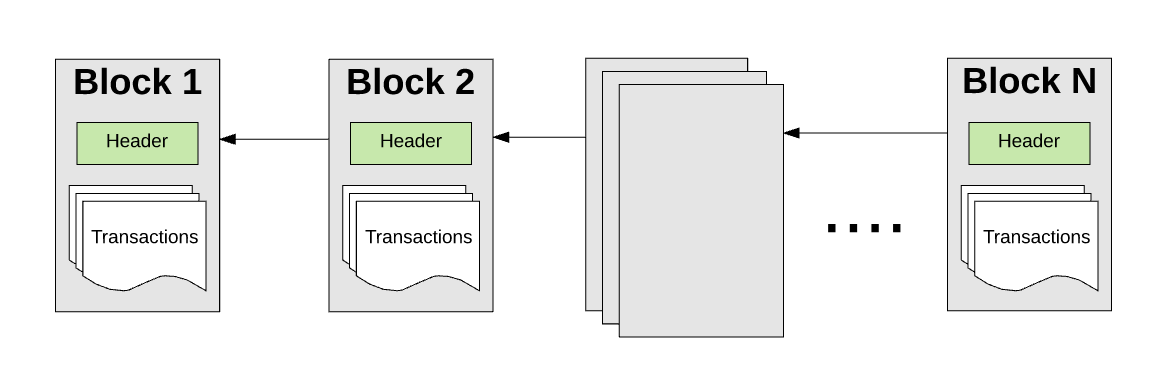
\includegraphics[width=70mm]{images/chain_of_blocks.png}
		\end{figure}

		Blockchain characteristics:
		\begin{itemize}
			\item Decentralization
			\item Trasparency
			\item Security
			\item Immutability
		\end{itemize}
		\textbf{Ethereum}: EVM, Smart Contracts and DAPP
    }
	
	
	\frame{
	    \frametitle{Process Mining}
		
		A \textbf{Business Process} is a collection of related and structured activities undertaken by one or more 
		organisations in order to pursue some particular goal.

		\vspace{16px}
		
		Process mining has the goal to discover, monitor and improve real processes by extracting knowledge from event logs 
		readily available in today's information systems.

		\vspace{16px}

		Three form of process mining:
		\begin{itemize}
			\item Process discovery
			\item Conformance checking
			\item Enhancement
		\end{itemize}
	}
	

	\frame{
		\frametitle{Discovery algorithms}
		Used discovery algorithms: 
		\begin{itemize}
			\item \textbf{Heuristic Miner}, it builds a Directly Follow Graph, filters noise based on ordering 
				relationship frequence

				\vspace{8px}

			\item \textbf{Inductive Miner}, it uses a divide-et-conquer approach, first it creates a DFG then it filter 
				infrequent dependencies and after that it applies cuts to the graph recursively

				\vspace{8px}

			\item \textbf{Split Miner}, produces a BPMN model in five steps:

			\begin{figure}[H]
				\centering
				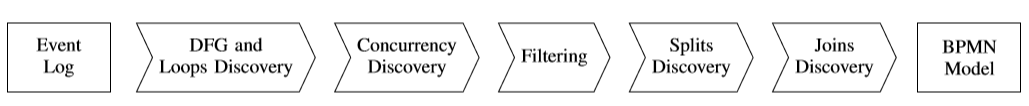
\includegraphics[width=110mm]{images/split_miner_steps.png}
			\end{figure}

		\end{itemize}
	}

	\frame{
		\frametitle{Case Studies}
		
		The methodology used for the case studies consists of several steps:
		
		\vspace{16px}

		\begin{figure}[t]
			\centering
			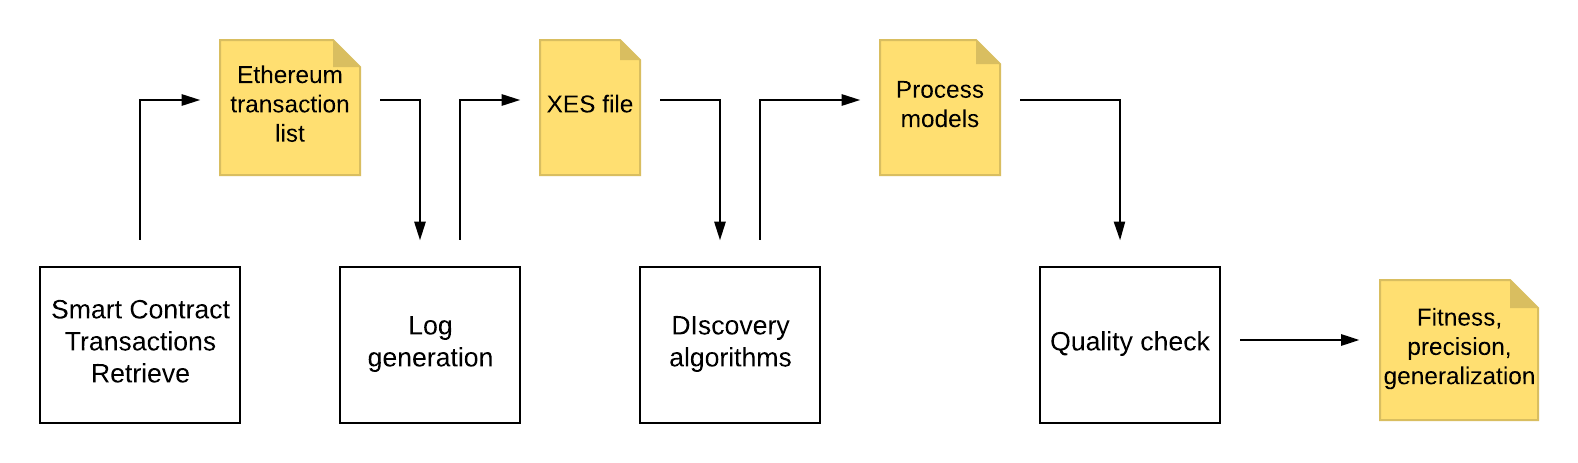
\includegraphics[width=120mm]{images/methodology.png}
		\end{figure}
	}


	\frame{
		\frametitle{RoToHive}

		\begin{figure}[t]
			\centering
			
\includegraphics[width=40mm]{images/rotohive.png}
		\end{figure}

		RotoHive is a new type of fantasy sports site that runs weekly tournaments.
		
		Model discovered with Heuristic Miner (the best algorithm in this case):

		\begin{figure}
			\centering
			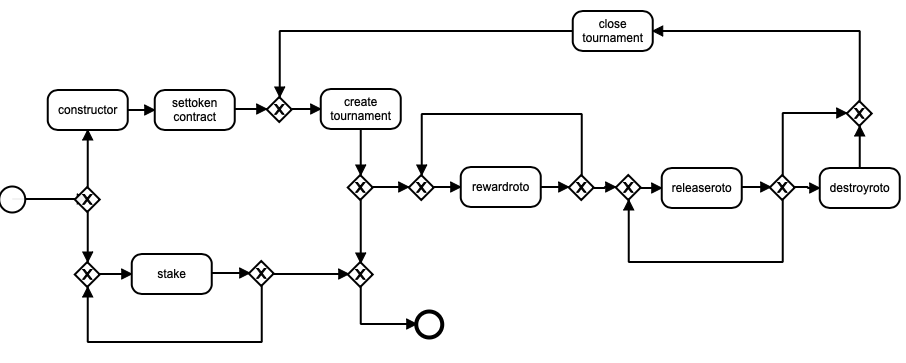
\includegraphics[width=90mm]{images/roto_heuristic.png}
		\end{figure}
	}

	\frame{
		\frametitle{Fomo 3D}

		This is a lottery game in which the last person to buy a key at the end of a round wins the jackpot!
		
		In this case, Split and Inductive Miner discovered the same model, better than Heuristic Miner one.

		\begin{figure}
			\centering
			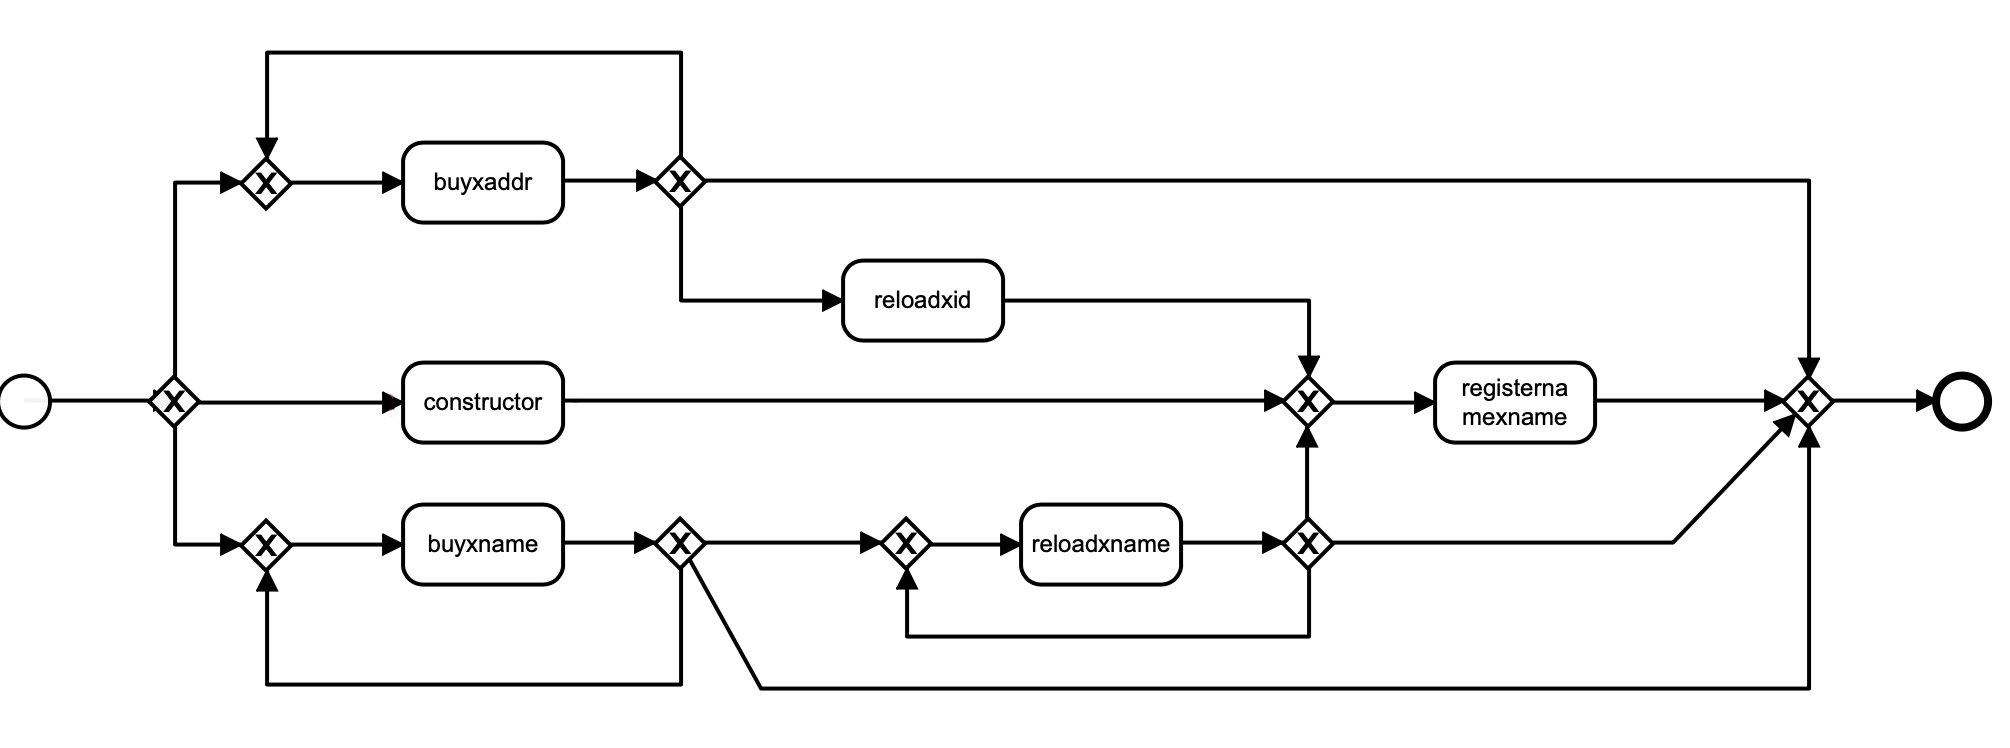
\includegraphics[width=110mm]{images/fomo_inductive.png}
		\end{figure}
	}

	\frame{
		\frametitle{IDEX}

		IDEX is a cryptocurrency exchange.
		Exchanges are applications that allows the user to deposit, withdraw or exchange cryptocurrencies.

		\begin{figure}
			\centering
			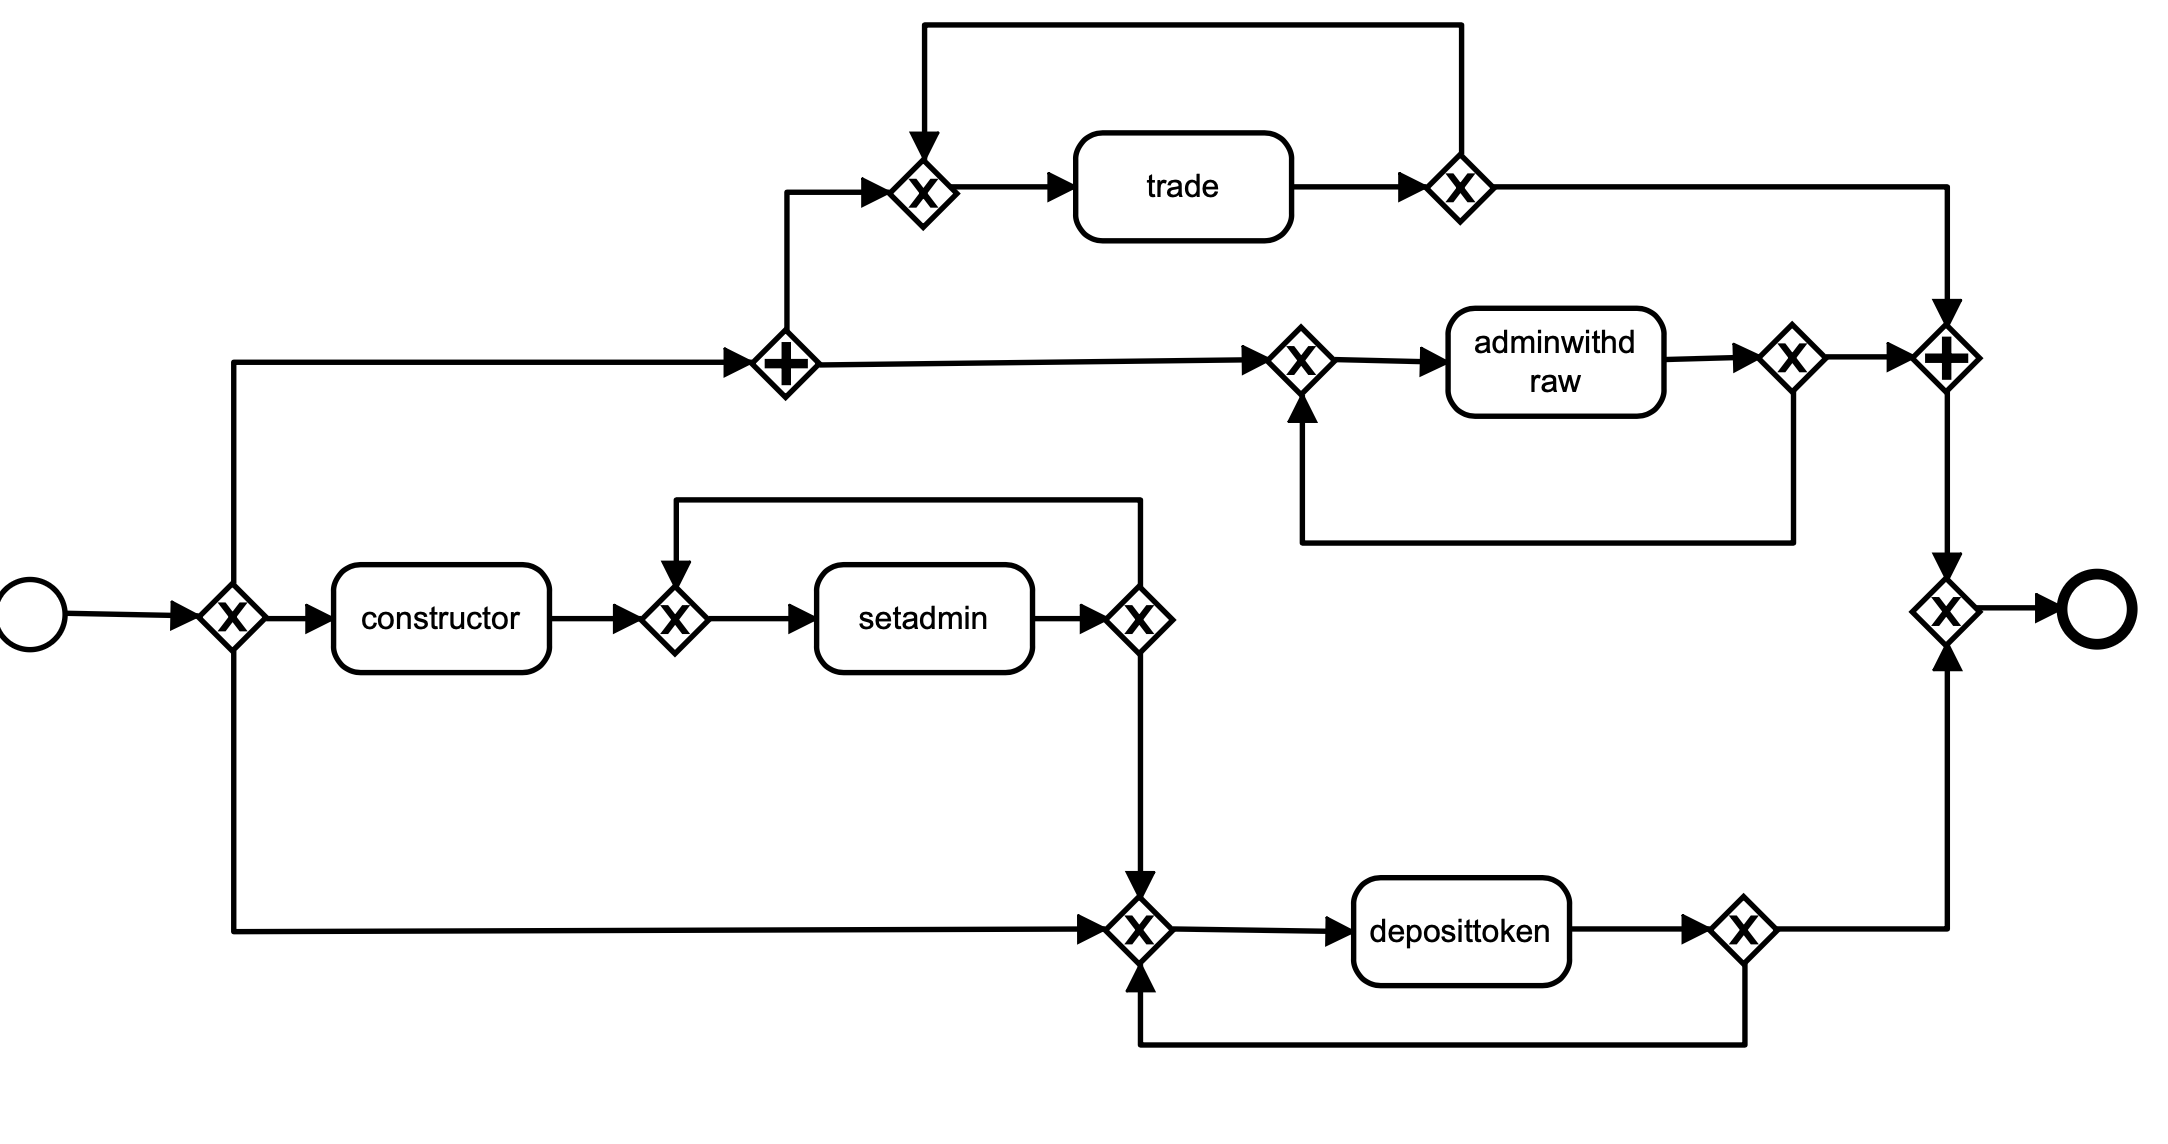
\includegraphics[width=110mm]{images/idex_inductive.png}
		\end{figure}
	}

	\frame{
		\frametitle{Quality measures}

		Quality measures obtained in the case studies with the three used algoritms:

		\begin{tiny}

			\begin{table}[htbp]
				\begin{tabular}{llllllllll}
												& \multicolumn{3}{l}{\textbf{Fitness}}                                                    & \multicolumn{3}{l}{\textbf{Precision}}                                                  & \multicolumn{3}{l}{\textbf{Generalization}}                                             \\
				{\color[HTML]{656565} Algorithm} & {\color[HTML]{656565} Roto} & {\color[HTML]{656565} Fomo} & {\color[HTML]{656565} IDEX} & {\color[HTML]{656565} Roto} & {\color[HTML]{656565} Fomo} & {\color[HTML]{656565} IDEX} & {\color[HTML]{656565} Roto} & {\color[HTML]{656565} Fomo} & {\color[HTML]{656565} IDEX} \\
				Split                      & 1                           & 0.97357                     & 0.99573                     & 0.20453                     & 0.47947                     & 0.22884                     & 0.99892                     & 0.96836                     & 0.99914                     \\
				Inductive                  & 0.99995                     & 0.97357                     & 0.99971                     & 0.60294                     & 0.47947                     & 0.48298                     & 0.99496                     & 0.96836                     & 0.99968                     \\
				Heuristic                  & 0.99940                     & 0.98710                     & 1                           & 0.49889                     & 0.48634                     & 0.32516                     & 0.99889                     & 0.87593                     & 0.99882                    
				\end{tabular}
			\end{table}

		\end{tiny}
	}


	\frame{
		\frametitle{Design and implementation}
		
		The system designed recreates the methodology used in the case studies analysis.

		\vspace{16px}

		The architecture of the Mining Framework: 

		\begin{figure}[t]
			\centering
			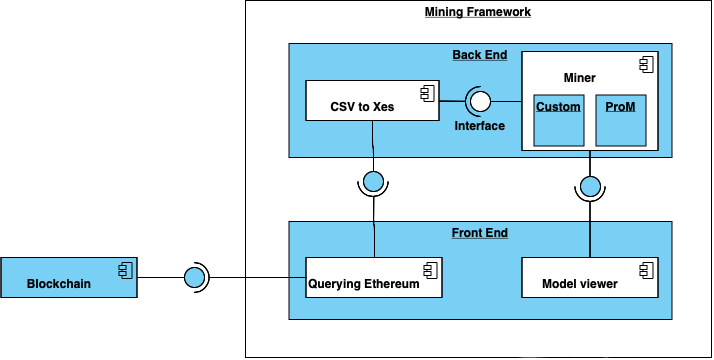
\includegraphics[width=80mm]{images/component_diagram.png}
		\end{figure}
	}


	\frame{
		\frametitle{Lessons learned}

		Sound models discovered and pretty good quality parameters measured.

		\vspace{16px}

		The three algorithms obtained similiar results. How well an algorithm fits a specific application domain depends from 
		the domain itself regardless the fact that it uses the Blockchain.

		\vspace{16px}

		The analysis infer the logic of the system. Can be used to increase solution quality, or understand how users interact with 
		a product.
	}


	\frame {
		\begin{center}
			Thanks for your attention!
		\end{center}
	}
    
\end{document}